%%%%%%%%%%%%%%%%%%%%%%%%%%%%%%%%%%%%%%%%%
% Jacobs Landscape Poster
% LaTeX Template
% Version 1.0 (29/03/13)
%
% Created by:
% Computational Physics and Biophysics Group, Jacobs University
% https://teamwork.jacobs-university.de:8443/confluence/display/CoPandBiG/LaTeX+Poster
%
% Further modified by:
% Nathaniel Johnston (nathaniel@njohnston.ca)
%
% This template has been downloaded from:
% http://www.LaTeXTemplates.com
%
% License:
% CC BY-NC-SA 3.0 (http://creativecommons.org/licenses/by-nc-sa/3.0/)
%
%%%%%%%%%%%%%%%%%%%%%%%%%%%%%%%%%%%%%%%%%

%----------------------------------------------------------------------------------------
%	PACKAGES AND OTHER DOCUMENT CONFIGURATIONS
%----------------------------------------------------------------------------------------

\documentclass[final]{beamer}

\usepackage[scale=1.24]{beamerposter} % Use the beamerposter package for laying out the poster

\usetheme{confposter} % Use the confposter theme supplied with this template

\setbeamercolor{block title}{fg=blue,bg=white} % Colors of the block titles
\setbeamercolor{block body}{fg=black,bg=white} % Colors of the body of blocks
\setbeamercolor{block alerted title}{fg=white,bg=dblue!70} % Colors of the highlighted block titles
\setbeamercolor{block alerted body}{fg=black,bg=dblue!10} % Colors of the body of highlighted blocks
% Many more colors are available for use in beamerthemeconfposter.sty

%-----------------------------------------------------------
% Define the column widths and overall poster size
% To set effective sepwid, onecolwid and twocolwid values, first choose how many columns you want and how much separation you want between columns
% In this template, the separation width chosen is 0.024 of the paper width and a 4-column layout
% onecolwid should therefore be (1-(# of columns+1)*sepwid)/# of columns e.g. (1-(4+1)*0.024)/4 = 0.22
% Set twocolwid to be (2*onecolwid)+sepwid = 0.464
% Set threecolwid to be (3*onecolwid)+2*sepwid = 0.708

\newlength{\sepwid}
\newlength{\onecolwid}
\newlength{\twocolwid}
\newlength{\threecolwid}
\setlength{\paperwidth}{48in} % A0 width: 46.8in
\setlength{\paperheight}{36in} % A0 height: 33.1in
\setlength{\sepwid}{0.02\paperwidth} % Separation width (white space) between columns
\setlength{\onecolwid}{0.31\paperwidth} % Width of one column
\setlength{\twocolwid}{0.464\paperwidth} % Width of two columns
\setlength{\threecolwid}{0.708\paperwidth} % Width of three columns
\setlength{\topmargin}{-0.5in} % Reduce the top margin size
%-----------------------------------------------------------

\usepackage{graphicx}  % Required for including images

\usepackage{booktabs} % Top and bottom rules for tables

%----------------------------------------------------------------------------------------
%	TITLE SECTION
%----------------------------------------------------------------------------------------

\title{The Math Exam/Educational Resources Wiki} % Poster title

\author{Carmen Bruni, Christina Koch, Bernhard Konrad, Mike Lindstrom, Iain Moyles, Will Thompson} % Author(s)

\institute{Department of Mathematics, The University of British Columbia} % Institution(s)

%----------------------------------------------------------------------------------------

\begin{document}

\addtobeamertemplate{block end}{}{\vspace*{2ex}} % White space under blocks
\addtobeamertemplate{block alerted end}{}{\vspace*{2ex}} % White space under highlighted (alert) blocks

\setlength{\belowcaptionskip}{2ex} % White space under figures
\setlength\belowdisplayshortskip{2ex} % White space under equations

\begin{frame}[t] % The whole poster is enclosed in one beamer frame

\begin{columns}[t] % The whole poster consists of three major columns, the second of which is split into two columns twice - the [t] option aligns each column's content to the top

\begin{column}{\sepwid}\end{column} % Empty spacer column

\begin{column}{\onecolwid} % The first column


%\begin{block}{Our Resource}

\begin{columns}
    \begin{column}{.5\textwidth}
        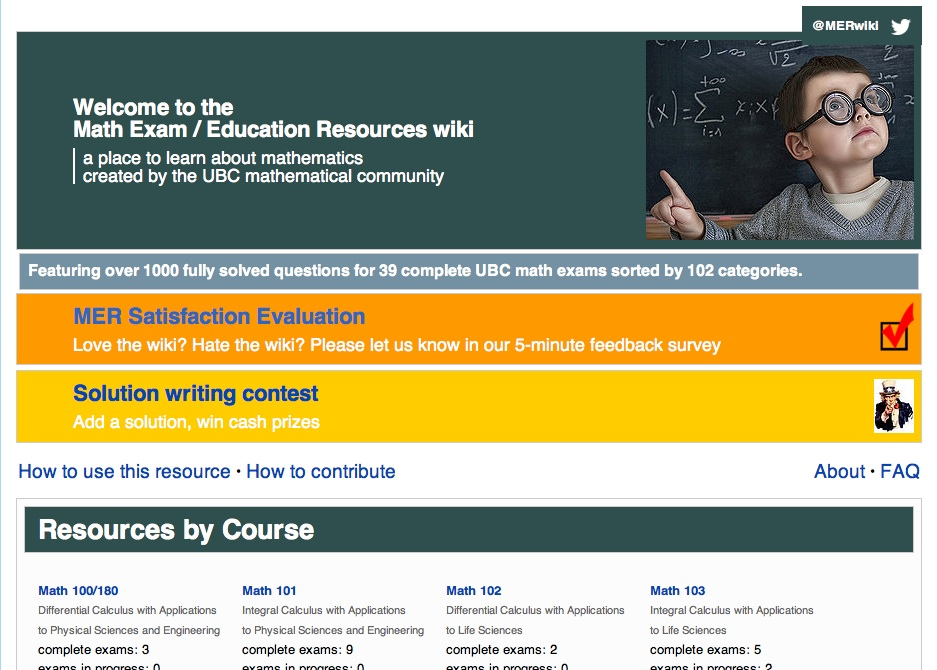
\includegraphics[width=\textwidth]{frontpage3.jpg}
    \end{column}
    \begin{column}{.5\textwidth}
    The Math Exam/Educational Resources wiki is a learning resource consisting of hints and solutions to previous UBC math exam questions, hosted on the UBC wiki.
    \end{column}
\end{columns}
%\end{block}

\begin{block}{Student Use}

This graph displays total clicks per day over the lifespan of the MER wiki. The horizontal lines indicate dates of final exams.

\smallskip

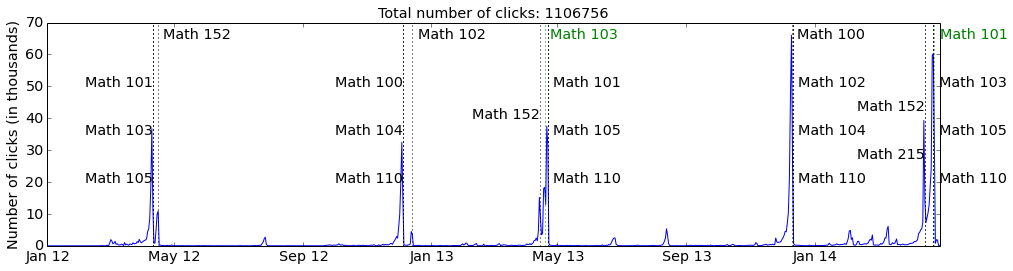
\includegraphics[width=\textwidth]{spikes.png}

\smallskip

\begin{center}
\hfill 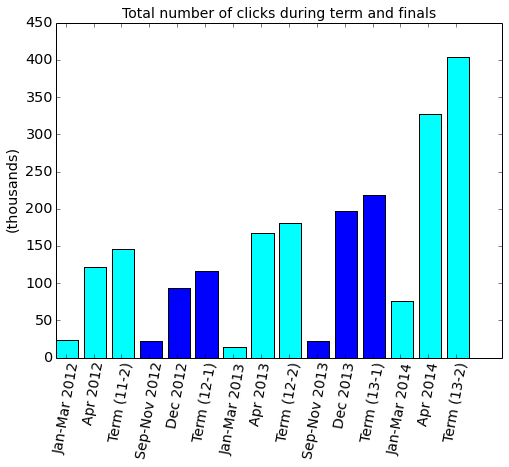
\includegraphics[width=.4\textwidth]{total_number_of_clicks_term_finals_bar.png} \hfill 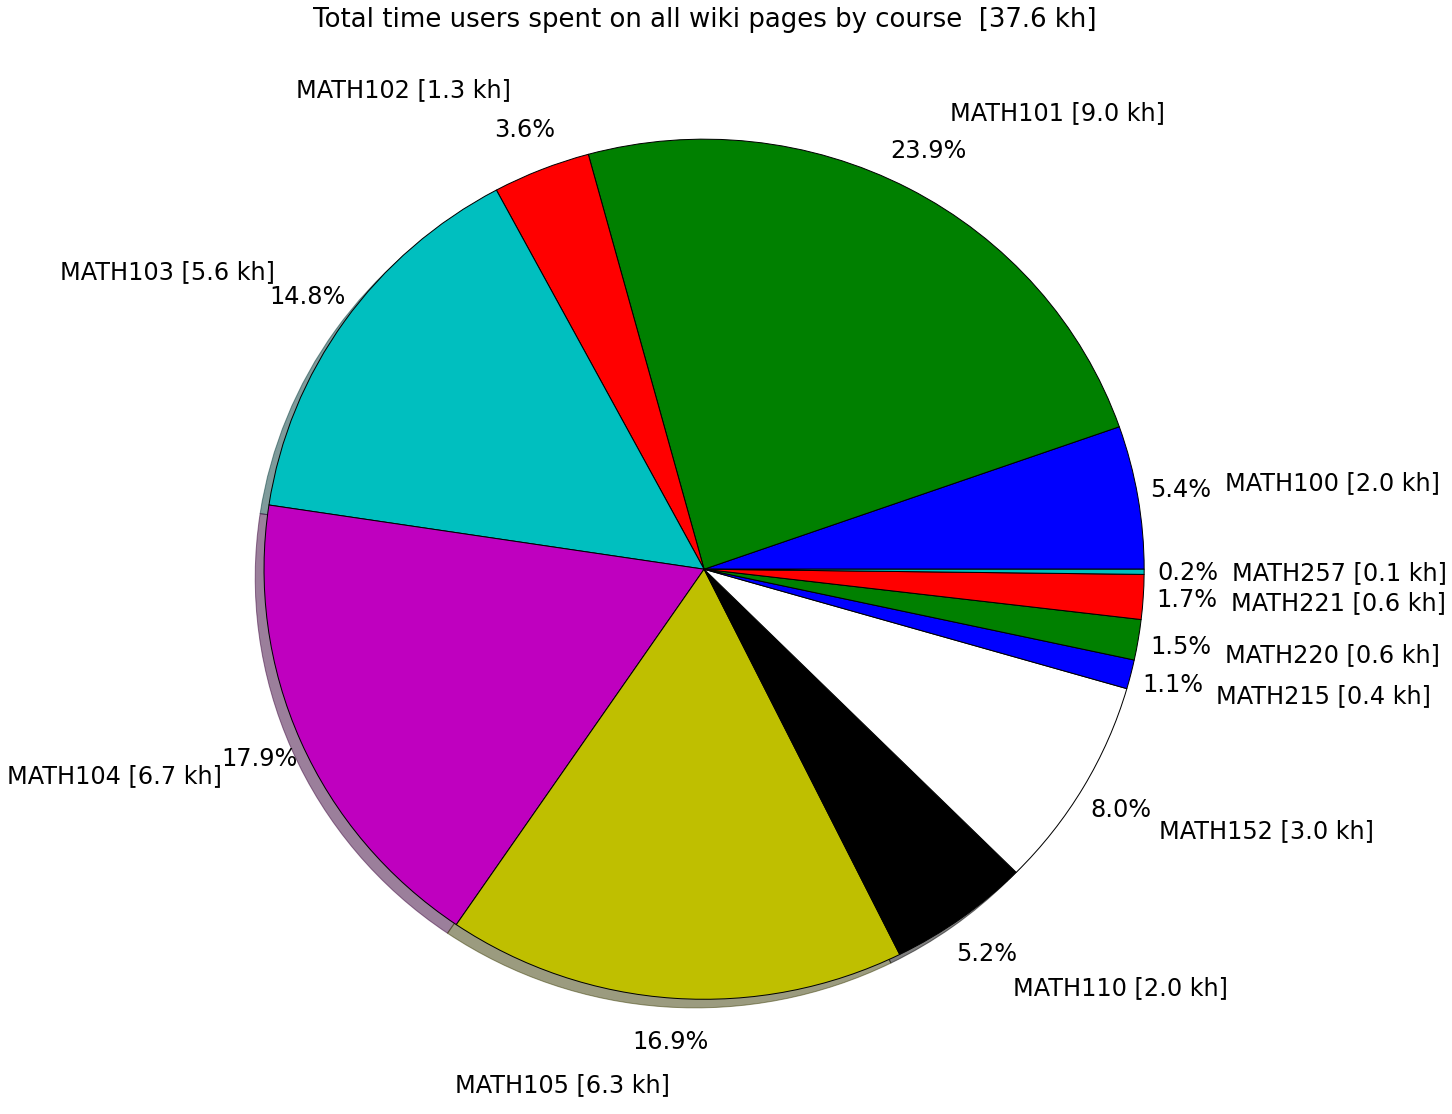
\includegraphics[width=.4\textwidth]{total_time_per_course.png} \hfill \mbox{}
\end{center}


\end{block}

\begin{block}{Brief History of the MER Wiki}
\begin{itemize}
      \item Math Department makes past exams publically available.
      \item Previous to the wiki, exam solutions were sold to students in hard copy.
      \item February 2012: math graduate students decided to write and publish exam solutions on the UBC wiki, making them free.
      \item Goal: improve content quality, system of delivery, student interaction.
	  \item The wiki structure is accessible, intuitive and simplifies collaboration.
\end{itemize}
\end{block}

\begin{block}{In 2 years, our volunteer team has...}
        \begin{itemize}
            \item Solved 44 complete exams, composed of over 1100 fully written hints and solutions from about 35 contributors.
            \item Added several dynamic and interactive features over time, like tagging system, course syllabus, rating bar, videos, and more.
                    \end{itemize}
\end{block}


\end{column} % End of the first column
%
%%----------------------------------------------------------------------------------------
%

\begin{column}{\sepwid}\end{column} % Empty spacer column

\begin{column}{\onecolwid} % Begin a column which is two columns wide (column 2)

\begin{alertblock}{Our Vision and Goals}
\begin{itemize}
\item Make this the best learning resource possible for undergraduate students taking math courses at UBC. %TODO: This is a littl vague. How about something more like "To provide detailed and high quality solutions that encourage and faciliate learning" or something like that?

\item Support instructors in the UBC Math Department.

\item Be a role model for similar initiatives in other departments.

\item Evaluate effectiveness and add features with TLEF funding.
\end{itemize}
\end{alertblock}


\begin{block}{Sample Question Page}
\begin{center}
\hfill
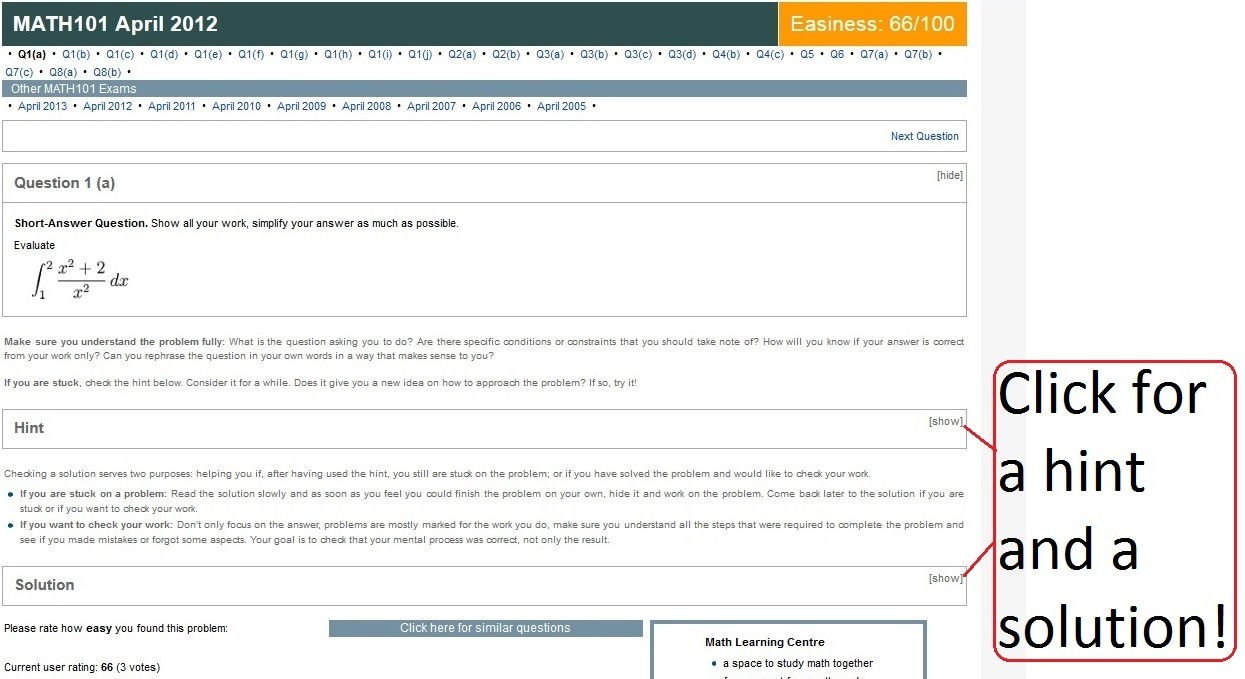
\includegraphics[width=.5\textwidth]{QuestionPage5.jpg} \hfill
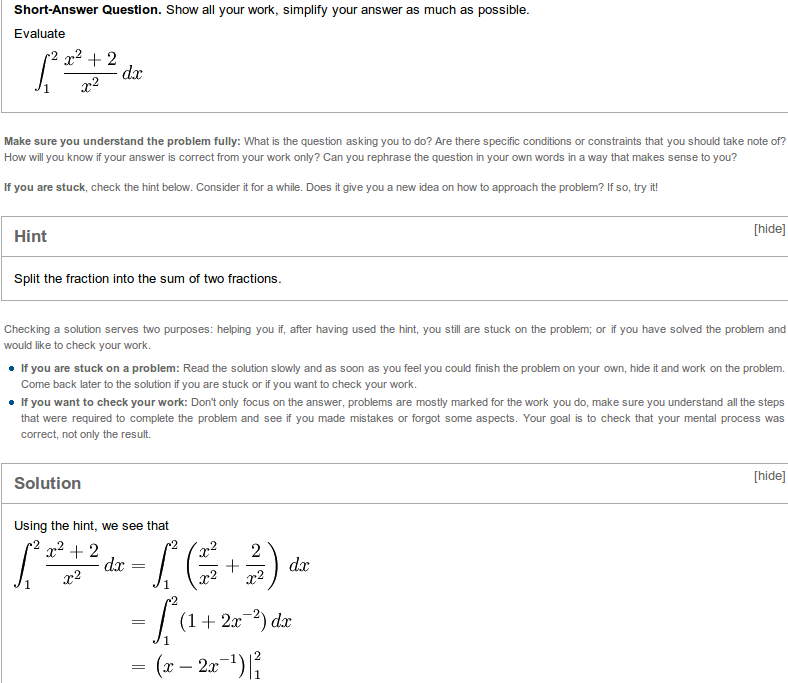
\includegraphics[width=.3\textwidth]{QuestionPage5_open.png} \hfill \mbox{}
\end{center}
\end{block}



\begin{block}{Peer-Reviewed Solutions}

All content is peer reviewed. This is a \emph{typical workflow:}

\medskip

\begin{itemize}
\item \textbf{Contributor A}: Adds question statement.
\item \textbf{Contributor B}: Reviews question statement. Also adds hint and solution.
\item \textbf{Contributor A}: Approves the hint, leaves a note on the discussion page that the solution should be more clear.
\item \textbf{Contributor C}: Edits solution.
\item \textbf{Contributor A}: Approves edited solution.
\end{itemize}

\end{block}


\vspace{-2cm}

\begin{center}
\begin{columns}[t]
\hfill
\begin{column}{.45\textwidth}
\begin{block}{Additional help}
For the April 2014 exam period we offered four free prep sessions on general study tips and how to use the wiki most effectively.

\bigskip

\begin{center}
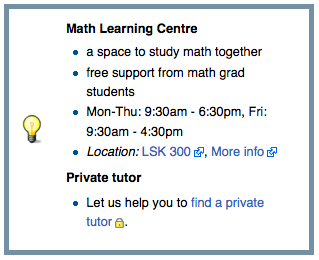
\includegraphics[width=.6\textwidth]{additional_help.png}
\end{center}
\end{block}
\end{column} \hfill
\begin{column}{.45\textwidth}
\begin{block}{Android app}
\begin{center}
%
\includegraphics[width=.3\textwidth]{en_app_rgb_wo_45.png}
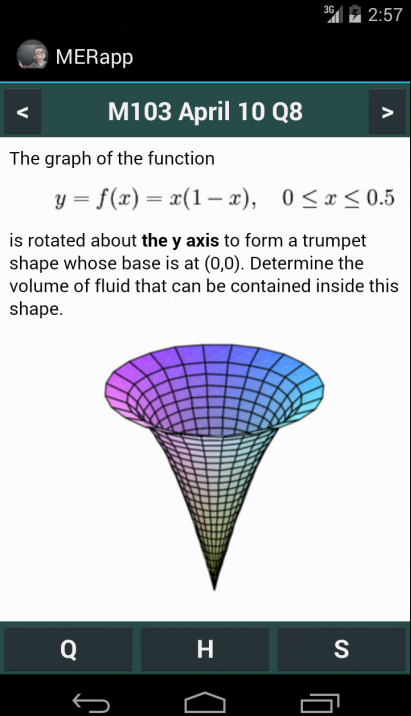
\includegraphics[width=.5\textwidth]{app_screen.png}
\end{center}
\end{block}
\end{column}
\hfill \mbox{}
\end{columns}
\end{center}


\end{column} % End of the second column
%
%%----------------------------------------------------------------------------------------
%

\begin{column}{\sepwid}\end{column} % Empty spacer column

\begin{column}{\onecolwid} % The third column


\begin{block}{Topic Tags and Dynamic Syllabus}

\begin{center}
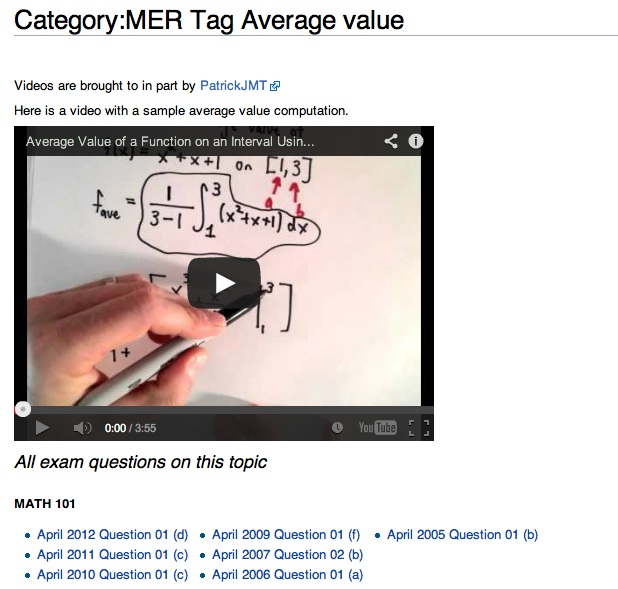
\includegraphics[width=.35\textwidth]{tag_with_video2.jpg} 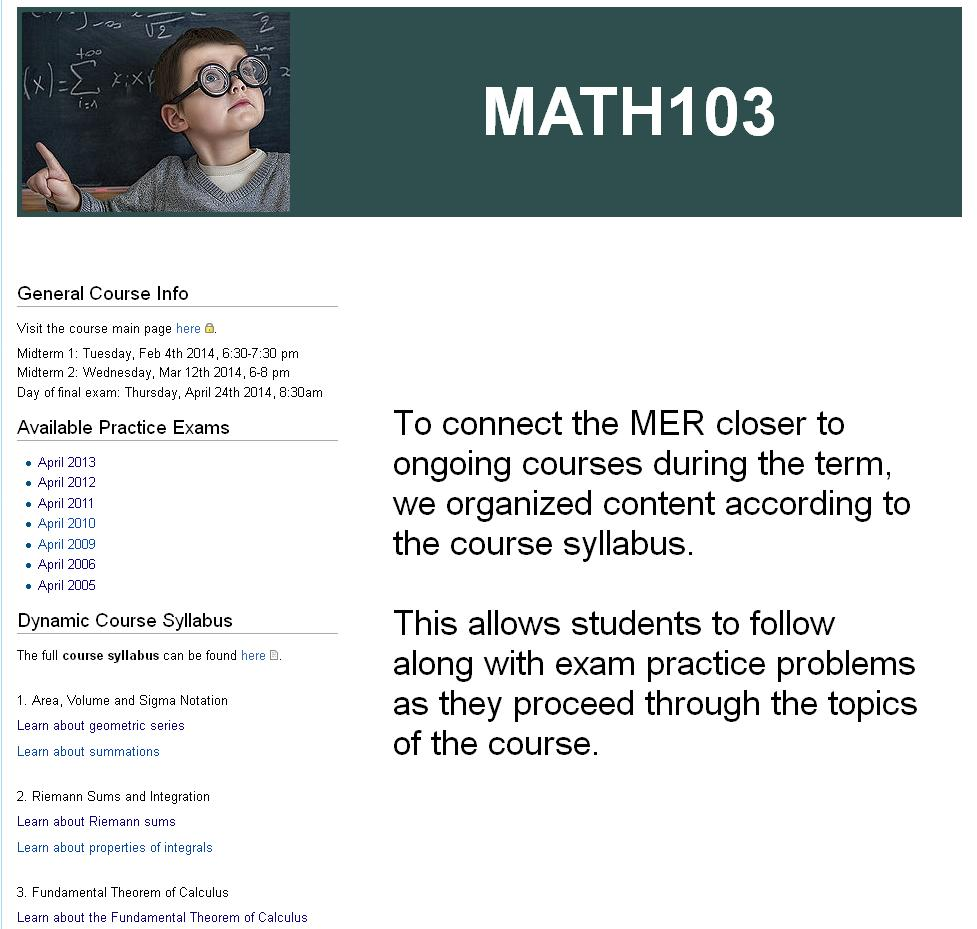
\includegraphics[width=.35\textwidth]{DynamicSyllabus.JPG}
\end{center}

\end{block}






\begin{block}{Rating Bar}

\begin{center}
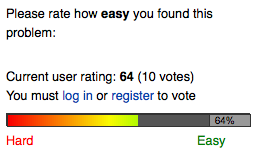
\includegraphics[width=.4\textwidth]{ratingBar.png} 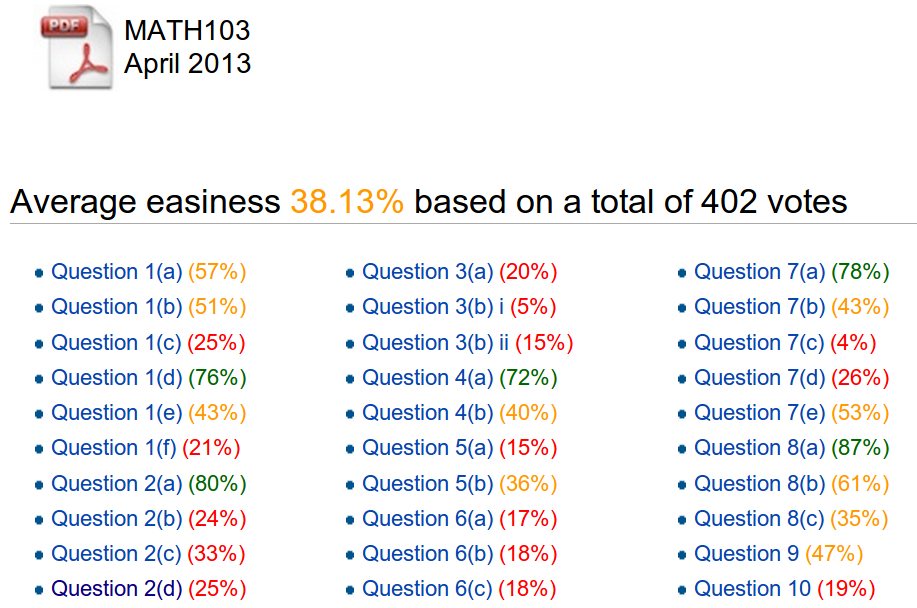
\includegraphics[width=.4\textwidth]{M103_exampage_rating.png}
\end{center}

\end{block}


\begin{block}{Student Questions and Comments}

\begin{center}
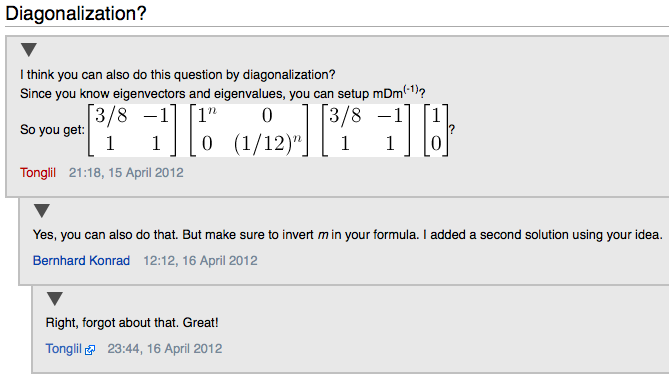
\includegraphics[width=.4\textwidth]{diagonalization.png} 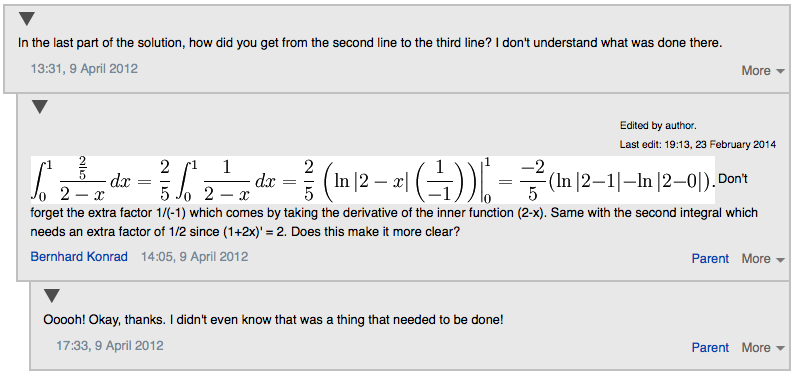
\includegraphics[width=.4\textwidth]{CommentQuestion3.png}
\end{center}

\end{block}

\vspace{-1.5cm}

\begin{block}{Solution Writing Contest}

In an first contest students suggested 22 new solutions to win cash prizes.

\begin{center}
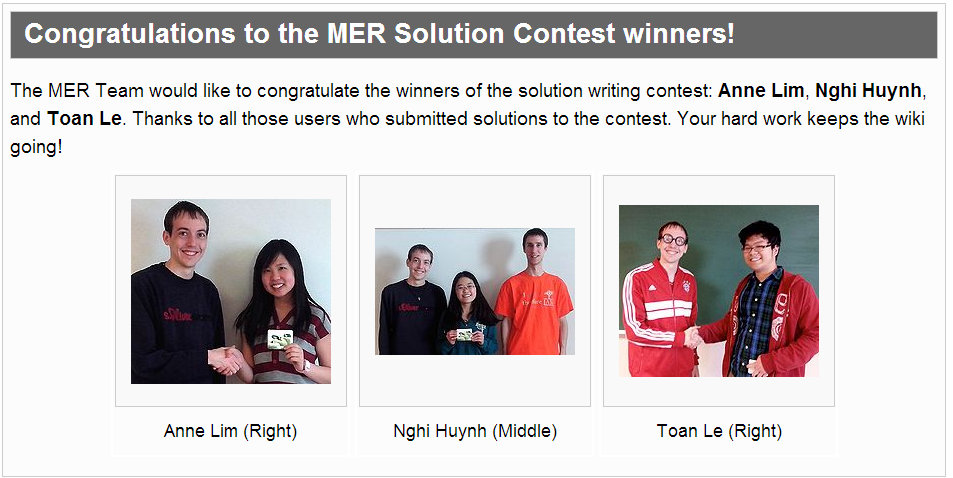
\includegraphics[width=.55\textwidth]{contest_winners.jpg}
\end{center}

\end{block}

%----------------------------------------------------------------------------------------
%	ACKNOWLEDGEMENTS
%----------------------------------------------------------------------------------------

%\setbeamercolor{block title}{fg=red,bg=white} % Change the block title color

\begin{block}{Acknowledgements}

\begin{columns}
\begin{column}{.2\textwidth}
\begin{center}

\includegraphics[width=.4\textwidth]{ubc_logo.jpg}
\end{center}
\end{column}
\begin{column}{.75\textwidth}
\small{\rmfamily{Recipients of a 2014-2015 TLEF-Flexible Learning Grant.}} \\ 

\small{\rmfamily{Thanks to Warren Code, Eric Cytrynbaum, Will Engle, Gillian Gerhard, Wes Maciejewski, Scott McMillan, Cindy Underhill, and the CTLT IT team for ongoing support and advice.}}
\end{column}
\end{columns}
 
\end{block}






%
%
%
%%----------------------------------------------------------------------------------------
%%	CONTACT INFORMATION
%%----------------------------------------------------------------------------------------
%
%\setbeamercolor{block alerted title}{fg=black,bg=norange} % Change the alert block title colors
%\setbeamercolor{block alerted body}{fg=black,bg=white} % Change the alert block body colors
%
%\begin{alertblock}{Contact Information}
%
%\begin{itemize}
%\item Web: \href{http://wiki.ubc.ca/Science:Math_Exam_Resources}{http://wiki.ubc.ca/Science:Math_Exam_Resources}
%\item Email: \href{mailto:mer-wiki@math.ubc.ca}{MER-wiki@math.ubc.ca}
%\end{itemize}
%
%\end{alertblock}

%\begin{center}
%\begin{tabular}{ccc}
%\includegraphics[width=0.4\linewidth]{logo.png} & \hfill & \includegraphics[width=0.4\linewidth]{logo.png}
%\end{tabular}
%\end{center}

%%----------------------------------------------------------------------------------------

\end{column} % End of the third column

\end{columns} % End of all the columns in the poster

\end{frame} % End of the enclosing frame

\end{document}

%sagemathcloud={"zoom_width":105}